\documentclass[11pt,a4paper]{article}

\usepackage[utf8]{inputenc}
\usepackage[margin=2.5cm]{geometry}
\usepackage{amsmath,amssymb}
\usepackage{graphicx}
\usepackage{booktabs}
\usepackage{enumitem}
\usepackage{hyperref}
\usepackage{natbib}
\usepackage{tikz}
\usetikzlibrary{arrows.meta,positioning,fit,backgrounds,calc}
\usepackage{xcolor}

\definecolor{memblue}{HTML}{DBEAFE}
\definecolor{trustorange}{HTML}{FED7AA}
\definecolor{beliefgreen}{HTML}{D1FAE5}
\definecolor{envpink}{HTML}{FCE7F3}
\definecolor{commpurple}{HTML}{EDE9FE}
\definecolor{normyellow}{HTML}{FEF9C4}
\definecolor{lockinpink}{HTML}{F5D0FE}
\definecolor{normred}{HTML}{FECACA}

\title{\textbf{Dual-Memory Cognitive Lock-in:\\Norm Emergence Through Experience, Predictive Confidence, and Normative Constraint}}
\author{}
\date{}

\begin{document}
\maketitle

\begin{abstract}
We present a dual-memory model of norm emergence in coordination games. Agents maintain two qualitatively distinct memory systems---an \emph{experience memory} (statistical, FIFO) and a \emph{normative memory} (rule-based, anomaly-tracked)---bridged by a single state variable, predictive confidence. High confidence stabilises experience-based beliefs through an expanded memory window (cognitive lock-in); low confidence makes agents susceptible to norm internalisation via a drift-diffusion process grounded in \citet{germar2014social}. Norms, once crystallised, constrain decisions, strengthen through conformity, erode through anomaly-triggered crises, and are enforced by high-conviction agents who observe violations. Three feedback loops---individual learning, social amplification, and normative pressure---emerge from this architecture without separate mechanisms, producing self-enforcing social norms from a cold start.
\end{abstract}

% =====================================================================
\section{Introduction}
% =====================================================================

Starting from a cold start---50-50 random strategy distribution, no shared history---how does randomness become a social norm? Not merely behavioural convergence, but a self-enforcing pattern sustained by mutual expectations \citep{bicchieri2006grammar}. Existing computational models have successfully explained convention emergence \citep{young1993evolution,shoham1997emergence}, norm persistence through conformist transmission \citep{boyd1985culture,henrich1998conformist}, enforcement via metanorms \citep{axelrod1986evolutionary}, adaptive cognitive effort \citep{epstein2001learning}, and the evolutionary origins of norm internalisation \citep{gavrilets2017collective}. We identify three structural distances between these contributions that the present model is designed to bridge.

\subsection{Three Structural Distances}

\paragraph{From exogenous to endogenous memory.}
In all prior models where memory exists, its length is a fixed parameter: Young's $m$ \citep{young1993evolution}, Shoham \& Tennenholtz's window \citep{shoham1997emergence}, Epstein's sample size \citep{epstein2001learning}. None implements the feedback loop that would make memory endogenous: better predictions $\to$ more confidence $\to$ longer memory $\to$ more stable beliefs $\to$ better predictions. Epstein comes closest---his agents reduce cognitive effort as norms strengthen---but this feedback runs in one direction only (norm $\to$ effort, not effort $\to$ norm formation), a consequence of maintaining a single representation of what to do.

\paragraph{From behavioural regularity to internalised rule.}
\citet{bicchieri2006grammar} distinguished empirical expectations (``what is done'') from normative expectations (``what should be done''); the is--ought gap \citep{hume1739treatise} means norms cannot be derived from experience alone. Yet all reviewed models use a single representation---a belief distribution, a propensity vector, or a utility parameter---that conflates the descriptive and the prescriptive. Young's and Shoham \& Tennenholtz's agents converge behaviourally without undergoing an internal state transition; Boyd \& Richerson's agents copy the majority without distinguishing ``most do $X$'' from ``one should do $X$.'' \citet{gavrilets2017collective} model internalisation explicitly through a genetic parameter~$\eta$, elegantly explaining the \emph{ultimate} cause, but the \emph{proximate} question---how an agent within a single generation transitions from ``no norm'' to ``internalised rule''---requires a cognitive process, not a fixed trait. Bridging this distance requires architecturally separating statistical beliefs from normative constraints.

\paragraph{From exogenous enforcement to emergent enforcement.}
When enforcement is modelled, it is supplied from outside the cognitive architecture: an evolved trait in Axelrod's metanorms \citep{axelrod1986evolutionary}, a strategic choice in Gavrilets \& Richerson \citep{gavrilets2017collective}, or absent entirely \citep{young1993evolution,epstein2001learning}. Bridging this distance requires a single cognitive variable---norm strength---that simultaneously governs compliance and triggers enforcement, so that rule-following and disapproval of violations arise from the same internal state.

\medskip
\noindent Review articles corroborate these distances: \citet{savarimuthu2011norm} note that most models address only one or two stages of the norm life cycle, while \citet{mahmoud2014review} identify cognitive norm internalisation and norm dissolution as minimally researched.

\subsection{This Model}

We address all three distances through a dual-memory architecture bridged by predictive confidence, detailed in Sections~\ref{sec:experience}--\ref{sec:enforcement_signal}. Table~\ref{tab:model_comparison} summarises the positioning.

\begin{table}[h]
\centering
\small
\begin{tabular}{lcccc}
\toprule
\textbf{Model} & \textbf{Adaptive memory} & \textbf{Is--ought distinction} & \textbf{Endogenous enforcement} & \textbf{Norm dissolution} \\
\midrule
Young (1993) & \texttimes & \texttimes & \texttimes & \texttimes \\
Boyd \& Richerson (1985) & \texttimes & \texttimes & \texttimes & \texttimes \\
Axelrod (1986) & \texttimes & \texttimes & genetic & \texttimes \\
Epstein (2001) & one-way & \texttimes & \texttimes & \texttimes \\
Gavrilets \& Richerson (2017) & \texttimes & genetic & strategic & \texttimes \\
\textbf{This model} & \textbf{bidirectional} & \textbf{architectural} & \textbf{emergent} & \textbf{crisis-based} \\
\bottomrule
\end{tabular}
\caption{Feature comparison with existing norm emergence models. ``Adaptive memory'': whether memory length responds to agent performance. ``Is--ought distinction'': whether the model architecturally separates empirical beliefs from normative rules. ``Endogenous enforcement'': whether enforcement arises from the same cognitive state that governs compliance. ``Norm dissolution'': whether norms can dissolve through accumulated contradictory evidence.}
\label{tab:model_comparison}
\end{table}

\subsection{Scope: Norms as Population-Level Phenomena}\label{sec:scope}

The model targets norm emergence in large anonymous populations, where norms are sustained by aggregate behavioural statistics and diffuse social pressure rather than by expectations of identified individuals. This corresponds to \citet{bicchieri2006grammar}'s \emph{generalised social expectations}---``people in this population expect and approve of doing~$A$''---as opposed to personal normative expectations directed at specific others. The architecture operationalises this distinction: experience memory captures empirical social expectations (what is done) as mean field beliefs \citep{mead1934mind}, normative memory captures normative social expectations (what should be done) as internalised rules, and enforcement signals carry anonymous social attitudes \citep{cialdini2004social}---all at the population level, without agent identification. The scope boundary this implies for small-group dynamics with reputation is discussed in Section~\ref{sec:summary}.

% =====================================================================
\section{Model Overview}
% =====================================================================

\subsection{Environment}

\begin{itemize}[itemsep=2pt]
    \item $N$ agents (even), strategy set $S = \{A, B\}$
    \item Pure coordination game: payoff 1 if both choose same strategy, 0 otherwise
    \item Each time step $t$: agents randomly paired, simultaneous strategy choice
    \item Agents observe partner's strategy (anonymous---always available regardless of $V$)
\end{itemize}

\paragraph{Global environment variables.} Two environment-level parameters control the information channels available to agents. These are \emph{not} agent state---they are uniform across the population and fixed for a given simulation run.

\begin{center}
\small
\begin{tabular}{llp{7cm}}
\toprule
\textbf{Variable} & \textbf{Type / Range} & \textbf{Semantics} \\
\midrule
$V$ (\emph{Visibility}) & $\mathbb{N}_0$ & Number of additional random interactions each agent observes per tick, beyond the direct partner. $V = 0$: agents observe \emph{only} their direct opponent---all social observation channels are closed. \\
$\Phi$ (\emph{SocialPressure}) & $[0, \infty)$ & Gain multiplier for enforcement broadcasts (Section~\ref{sec:enforcement_signal}). $\Phi = 0$: all normative signalling is disabled---no enforcement signals are sent or received. $\Phi = 1$: baseline enforcement. $\Phi > 1$: amplified social pressure. \\
\bottomrule
\end{tabular}
\end{center}

\noindent These variables are \emph{not} varied in the default 2$\times$2 factorial (Section~\ref{sec:experimental}). They serve as experimental levers for ablation studies that independently control social observation and enforcement pressure (Section~\ref{sec:ablation}).

\subsection{Per-Tick Execution Order}

Each tick follows a fixed synchronous pipeline. All interaction outcomes are collected before updates are applied in synchronized passes, avoiding within-tick order effects. Figure~\ref{fig:tick_dataflow} shows the six stages with the variables written and read at each stage.

\begin{figure}[h]
\centering
\begin{tikzpicture}[
    >=Stealth,
    step/.style={draw, rounded corners, minimum width=5.2cm, minimum height=0.7cm, align=center, font=\small},
    var/.style={font=\scriptsize, text width=6cm, align=left},
    every node/.style={font=\small}
]
% Steps (left column)
\node[step, fill=envpink]     (s1) at (0, 0)    {1.\ Pair and Action};
\node[step, fill=memblue]     (s2) at (0,-1.2)  {2.\ Observe ($V$) and Memory Update};
\node[step, fill=trustorange]  (s3) at (0,-2.4)  {3.\ Confidence Update};
\node[step, fill=normred]      (s4) at (0,-3.6)  {4.\ Normative Update (DDM / Anomaly)};
\node[step, fill=normyellow]   (s5) at (0,-4.8)  {5.\ Enforcement Broadcast ($\Phi$)};
\node[step, fill=beliefgreen]  (s6) at (0,-6.0)  {6.\ Metrics};

% Arrows
\foreach \i/\j in {s1/s2, s2/s3, s3/s4, s4/s5, s5/s6}
    \draw[->, thick] (\i) -- (\j);

% Right column: variables written/read at each stage
\node[var] at (5.8, 0)    {\textbf{Write:} $s_i, s_j$ (actions via Eq.~\ref{eq:prob_matching})};
\node[var] at (5.8,-1.2)  {\textbf{Write:} $M^E_i$, $\mathbf{b}^{\text{exp}}$ \quad \textbf{Gate:} $V$};
\node[var] at (5.8,-2.4)  {\textbf{Write:} $C_i$ (Eq.~\ref{eq:confidence_update}) \quad \textbf{Read:} $w_i\!=\!f(C_i)$ (Eq.~\ref{eq:window})};
\node[var] at (5.8,-3.6)  {\textbf{Write:} $e_i$, $\sigma_i$, $a_i$ (Eqs.~\ref{eq:drift}--\ref{eq:crisis})};
\node[var] at (5.8,-4.8)  {\textbf{Write:} $p_i$ broadcast (Eq.~\ref{eq:signal_push}) \quad \textbf{Gate:} $\Phi$};
\node[var] at (5.8,-6.0)  {\textbf{Read:} all; no state written};
\end{tikzpicture}
\caption{Single-tick dataflow. Left: execution stages in fixed order; environment gates ($V$, $\Phi$) annotated where they modulate information flow. Right: variables written/read at each stage, with equation references. Use this figure to trace where any symbol first appears and where it is consumed.}
\label{fig:tick_dataflow}
\end{figure}

\subsection{Agent State}

Each agent $i$ at time $t$ maintains:

\begin{table}[h]
\centering
\begin{tabular}{llll}
\toprule
\textbf{Component} & \textbf{Symbol} & \textbf{Type} & \textbf{Role} \\
\midrule
Pred.\ confidence & $C_i(t) \in [0, 1]$ & State variable & Bridges both memories \\
Experience memory & $M_i^E(t)$ & FIFO queue & Statistical belief formation \\
Normative memory & $M_i^N$ & Rule + strength + anomalies & Decision constraint \\
\bottomrule
\end{tabular}
\end{table}

\subsection{Architectural Principle}

Predictive confidence $C_i(t) \in [0,1]$ measures agent $i$'s confidence in the predictability of the social environment. It answers: \emph{``How reliably can I predict what will happen in my next interaction?''} This is distinct from interpersonal trust \citep{rotter1967new} (directed at specific partners) or institutional trust \citep{luhmann1979trust} (directed at organisations). It is a purely epistemic variable---an agent's meta-cognitive assessment of environmental stability, closely related to the inverse of perceived volatility in \citet{behrens2007learning}. $C_i$ governs pre-crystallisation processes (memory window, DDM drift, signal susceptibility) but \emph{not} post-crystallisation compliance, which is governed by norm strength $\sigma_i$ (Section~\ref{sec:decision}).

Predictive confidence is \textbf{not} a parameter of either memory system. It is a single state variable whose semantic interpretation naturally produces two functional roles in the cognitive layer:

\begin{center}
\begin{tabular}{lll}
\toprule
\textbf{Confidence level} & \textbf{Meaning} & \textbf{Consequence} \\
\midrule
Low ($< 0.3$) & ``I cannot predict this environment'' & Short window; own experience unreliable $\to$ susceptible to norm internalisation \\
Medium ($0.3$--$0.7$) & ``I can roughly predict'' & Moderate window; norm provides useful constraint \\
High ($> 0.7$) & ``I can reliably predict'' & Long window; own experience sufficient $\to$ can override norm \\
\bottomrule
\end{tabular}
\end{center}

Figure~\ref{fig:dual_memory} provides an overview of the architecture before the detailed specifications that follow.

\begin{figure}[h]
\centering
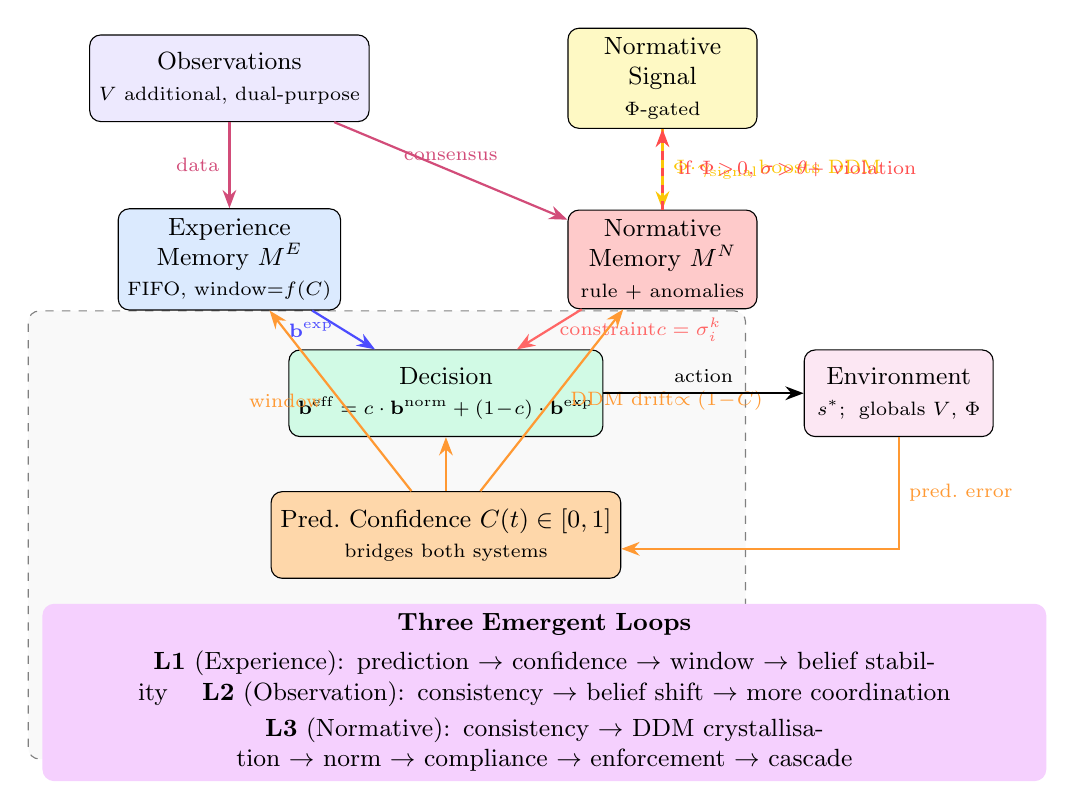
\begin{tikzpicture}[
    >=Stealth,
    box/.style={draw, rounded corners, minimum width=2.4cm, minimum height=1.1cm, align=center, font=\small},
    smallbox/.style={draw, rounded corners, minimum width=1.8cm, minimum height=0.8cm, align=center, font=\scriptsize},
    arrow/.style={->, thick},
    label/.style={font=\scriptsize, midway},
    every node/.style={font=\small}
]

% ---- Two Memory Systems ----
\node[box, fill=memblue] (expmem) at (-2, 3.5) {Experience\\Memory $M^E$\\{\scriptsize FIFO, window=$f(C)$}};
\node[box, fill=normred] (normmem) at (3.5, 3.5) {Normative\\Memory $M^N$\\{\scriptsize rule + anomalies}};

% ---- Trust ----
\node[box, fill=trustorange, minimum width=3cm] (trust) at (0.75, 0) {Pred.\ Confidence $C(t) \in [0,1]$\\{\scriptsize bridges both systems}};

% ---- Decision ----
\node[box, fill=beliefgreen] (decision) at (0.75, 1.8) {Decision\\{\scriptsize $\mathbf{b}^{\text{eff}} = c \cdot \mathbf{b}^{\text{norm}} + (1\!-\!c) \cdot \mathbf{b}^{\text{exp}}$}};

% ---- Observations ----
\node[box, fill=commpurple] (obs) at (-2, 5.8) {Observations\\{\scriptsize $V$ additional, dual-purpose}};

% ---- Normative Signal ----
\node[box, fill=normyellow] (signal) at (3.5, 5.8) {Normative\\Signal\\{\scriptsize $\Phi$-gated}};

% ---- Environment ----
\node[box, fill=envpink] (env) at (6.5, 1.8) {Environment\\{\scriptsize $s^*$;\; globals $V$, $\Phi$}};

% ---- Agent boundary ----
\begin{scope}[on background layer]
    \node[draw=gray, dashed, rounded corners, fill=gray!5,
          fit=(expmem)(normmem)(trust)(decision),
          inner sep=14pt, label={[font=\small\bfseries]above:AGENT}] {};
\end{scope}

% ---- Internal arrows ----
\draw[arrow, blue!70] (expmem) -- node[label, left] {$\mathbf{b}^{\text{exp}}$} (decision);
\draw[arrow, red!60] (normmem) -- node[label, right] {constraint\\{\scriptsize $c=\sigma_i^k$}} (decision);
\draw[arrow, orange!80] (trust) -- node[label, left, xshift=-3pt] {window} (expmem);
\draw[arrow, orange!80] (trust) -- node[label, right, xshift=3pt] {DDM drift\\{\scriptsize $\propto(1\!-\!C)$}} (normmem);
\draw[arrow, orange!80] (trust) -- (decision);

% ---- Environment arrows ----
\draw[arrow] (decision) -- node[label, above] {action} (env);
\draw[arrow, orange!80] (env) |- node[label, near start, right] {pred.\ error} ([yshift=-5pt]trust.east);

% ---- Observation arrows ----
\draw[arrow, purple!70] (obs) -- node[label, left] {data} (expmem);
\draw[arrow, purple!70] (obs) -- node[label, above] {consensus} (normmem);

% ---- Signal arrows ----
\draw[arrow, yellow!60!orange, thick] (signal) -- node[label, right] {$\Phi \!\cdot\! \gamma_{\text{signal}}$\\{\scriptsize boosts DDM}} (normmem);

% ---- Enforcement arrow (from decision out) ----
\draw[arrow, red!70, dashed] (normmem) -- node[label, right, xshift=2pt] {if $\Phi\!>\!0$,\;$\sigma\!>\!\theta$\\+ violation} (signal);

% ---- Lock-in annotation ----
\node[draw=lockinpink, fill=lockinpink, rounded corners, text width=12.5cm, align=center, font=\small] at (2, -2) {
    \textbf{Three Emergent Loops}\\[3pt]
    \textbf{L1} (Experience): prediction $\to$ confidence $\to$ window $\to$ belief stability \quad
    \textbf{L2} (Observation): consistency $\to$ belief shift $\to$ more coordination\\[2pt]
    \textbf{L3} (Normative): consistency $\to$ DDM crystallisation $\to$ norm $\to$ compliance $\to$ enforcement $\to$ cascade
};

\end{tikzpicture}
\caption{Dual-memory architecture. Predictive confidence bridges experience memory (statistical, FIFO) and normative memory (rule-based, anomaly-tracked). Observations ($V$ per tick beyond the direct partner) feed both systems simultaneously. Enforcement signals are violation-triggered, norm-strength-gated, and scaled by $\Phi$. When $V = 0$ or $\Phi = 0$, the corresponding channel is disabled (see Section~\ref{sec:ablation}).}
\label{fig:dual_memory}
\end{figure}

\subsection{Bridge Variables}\label{sec:bridge}

The subsystems communicate through exactly three bridge variables. All other state is internal to each layer. This table serves as a roadmap for Sections~\ref{sec:experience}--\ref{sec:enforcement_signal}: each section defines one layer and specifies how it writes or reads these bridge variables.

\begin{center}
\small
\texttt{Experience layer} $\;\xrightarrow{\;C_i\;}\;$ \texttt{Normative layer} $\;\xrightarrow{\;\sigma_i\;}\;$ \texttt{Decision layer} $\;\xleftarrow{\;p_i\;}\;$ \texttt{Enforcement}
\end{center}

\begin{table}[h]
\centering
\small
\begin{tabular}{lp{3.8cm}p{4.5cm}p{3.5cm}}
\toprule
\textbf{Variable} & \textbf{Written by} & \textbf{Read by} & \textbf{Semantics} \\
\midrule
$C_i$ & Confidence update (Eq.~\ref{eq:confidence_update}) & Window size (Eq.~\ref{eq:window}), DDM drift (Eq.~\ref{eq:drift}), Signal sensitivity (Eq.~\ref{eq:signal_push}) & ``How predictable is my environment?'' \\
$\sigma_i$ & Crystallisation (Eq.~\ref{eq:crystal}), Strengthening (Eq.~\ref{eq:strengthen}), Crisis (Eq.~\ref{eq:crisis}) & Compliance (Eq.~\ref{eq:compliance}), Enforcement gating (Eq.~\ref{eq:violation_response}) & ``How constraining is my norm?'' \\
$p_i$ & Enforcement broadcast (Eq.~\ref{eq:violation_response}) & DDM evidence update (Eq.~\ref{eq:ddm}) & ``What does the group say I should do?'' \\
\bottomrule
\end{tabular}
\caption{Bridge variables connecting the three subsystems. Three bridge variables for three subsystems indicates low coupling; the pipeline check ($\leq 5$) is satisfied.}
\label{tab:bridge}
\end{table}

\noindent In addition to the three bridge variables, the environment-level parameters $V$ and $\Phi$ modulate information flow: $V$ gates the observation channel feeding both memories (Stages~2 and~4), while $\Phi$ gates the enforcement broadcast channel (Stage~5). These are not bridge variables---they do not carry information between subsystems---but they control whether specific inter-subsystem channels are active.

% =====================================================================
\section{Experience Memory and Cognitive Lock-in}\label{sec:experience}
% =====================================================================

Experience memory is the statistical layer. It stores the direct interaction record and (when $V > 0$) additional observation data, producing a belief distribution over strategies.

\begin{center}
\small
\begin{tabular}{llll}
\toprule
\textbf{Symbol} & \textbf{Range} & \textbf{Defined in} & \textbf{Role} \\
\midrule
$\mathbf{b}^{\text{exp}}$ & $[0,1]^2$ & This section & Belief from experience \\
$C_i$ & $[0,1]$ & This section & Predictive confidence (\textbf{bridge} $\to$ normative layer) \\
$w_i$ & $\{2,\ldots,6\}$ & This section & Effective memory window $= f(C_i)$ \\
$\alpha, \beta$ & params & Table~\ref{tab:params} & Confidence increase / decrease rates \\
\bottomrule
\end{tabular}
\end{center}

\subsection{Belief Formation}

\begin{equation}
b_A = \frac{n_A}{|M'^E_i(t)|}, \quad b_B = 1 - b_A
\end{equation}
where $n_A$ is the count of strategy $A$ in the effective window. Default: $[0.5, 0.5]$.

\subsection{Action Selection (Probability Matching)}

\begin{equation}\label{eq:prob_matching}
P(s_i = A) = b_A^{\text{eff}}, \quad P(s_i = B) = b_B^{\text{eff}}
\end{equation}
where $\mathbf{b}^{\text{eff}}$ is the effective belief after normative constraint (Section~\ref{sec:decision}).

\subsection{Confidence Update}

\begin{equation}\label{eq:confidence_update}
C_i(t\!+\!1) = \begin{cases}
C_i(t) + \alpha (1 - C_i(t)) & \text{if prediction correct} \\
C_i(t) (1 - \beta) & \text{if prediction wrong}
\end{cases}
\end{equation}

Prior to each interaction, agent $i$ forms a prediction $\hat{s}_j$ of its partner's strategy. A prediction is \emph{correct} when $\hat{s}_j = s_j$ (the partner's actual choice), regardless of agent $i$'s own action or the resulting payoff. In pure coordination games, prediction accuracy and coordination success are highly correlated, but they are conceptually independent: an agent may predict correctly yet fail to coordinate (e.g., due to stochastic action selection), or coordinate by chance despite an incorrect prediction. This distinction becomes substantive when generalising to asymmetric games, where predicting a partner's behaviour and achieving a favourable outcome may diverge systematically.

Asymmetric by design \citep{slovic1993perceived}: predictive confidence builds slowly through successful predictions (additive, saturating) and collapses quickly after prediction failures (multiplicative). This mirrors the empirical finding that perceived environmental stability is easier to disconfirm than to establish. Steady state:
\begin{equation}\label{eq:confidence_steady}
C^* = \frac{p\alpha}{p\alpha + (1-p)\beta}
\end{equation}

\subsection{Confidence--Memory Window Linkage}

\begin{equation}\label{eq:window}
w_i(t) = \text{base} + \lfloor C_i(t) \times (\text{max} - \text{base}) \rfloor
\end{equation}

The upper bound $\text{max} = 6$ follows \citet{hertwig2010decisions} and \citet{nevo2012bi}, whose BI-SAW model---winner of the 2010 Market Entry Prediction Competition---found that agents recall only the most recent 6 trials.

\subsection{The Cognitive Lock-in Mechanism}

\begin{center}
Majority forms (drift) $\to$ prediction accuracy $\uparrow$ $\to$ confidence $\uparrow$ $\to$ window $\uparrow$ $\to$ beliefs stabilise $\to$ norm resilience $\uparrow$
\end{center}

Probability matching is behaviourally neutral: any norm emergence is attributable to the memory mechanism, not behavioural biases. \textbf{Limitation}: convergence is slow without social amplification.

% =====================================================================
\section{Normative Memory}
% =====================================================================

Normative memory is qualitatively different from experience memory. It stores a \emph{rule}, not data. It acts as a \emph{constraint} on decisions, not a source of beliefs.

\begin{center}
\small
\begin{tabular}{llll}
\toprule
\textbf{Symbol} & \textbf{Range} & \textbf{Defined in} & \textbf{Role} \\
\midrule
$r_i$ & $S \cup \{\varnothing\}$ & This section & Norm rule (or none) \\
$\sigma_i$ & $[0,1]$ & This section & Norm strength (\textbf{bridge} $\to$ decision layer) \\
$a_i$ & $\mathbb{N}$ & This section & Anomaly counter \\
$e_i$ & $\mathbb{R}$ & This section & DDM evidence accumulator \\
\midrule
\multicolumn{4}{l}{\emph{Read from other layers:} $C_i$ (experience layer), $p_i$ (enforcement)} \\
\bottomrule
\end{tabular}
\end{center}

\subsection{Structure}

\begin{equation}
M_i^N = \left(\, r_i \in S \cup \{\varnothing\},\;\; \sigma_i \in [0,1],\;\; a_i \in \mathbb{N},\;\; e_i \in \mathbb{R} \,\right)
\end{equation}

\begin{itemize}[itemsep=2pt]
    \item $r_i$: the norm (which strategy is ``the rule''), or $\varnothing$ if no norm has formed
    \item $\sigma_i$: norm strength (how constraining the rule is)
    \item $a_i$: anomaly count (accumulated violations observed)
    \item $e_i$: DDM evidence accumulator (pre-crystallisation)
\end{itemize}

Normative memory is \textbf{not FIFO}. It does not slide, decay, or reweight. Once formed, the norm persists as a discrete rule until overthrown through crisis. Observations feed both memory systems simultaneously: experience memory extracts \emph{frequencies}; normative memory detects \emph{consensus} (pre-crystallisation) or \emph{violations} (post-crystallisation).

\subsection{Norm Formation: Signed Two-Boundary Drift-Diffusion}\label{sec:formation}

Norm formation follows a \emph{signed} two-boundary drift-diffusion process \citep{germar2014social,germar2019learning}. Observations accumulate as strategy-directional noisy evidence; a norm crystallises when accumulated evidence crosses either boundary.

\paragraph{Theoretical basis.} \citet{germar2014social} showed that social norms alter the drift rate in perceptual decision-making, using a standard two-boundary DDM where subjects could shift toward either response. \citet{germar2019learning} demonstrated that this alteration \emph{persists} after social influence is removed---norms are internalised as a persistent cognitive bias, not a transient effect. \citet{tenenbaum2011grow} established that rule learning from examples is fundamentally probabilistic (Bayesian inference over rule hypotheses).

\paragraph{Observation set.} Let $\mathcal{O}_i(t)$ denote agent $i$'s observation set at tick $t$: the direct partner's strategy plus $V$ randomly sampled interaction outcomes, giving $|\mathcal{O}_i(t)| = 1 + V$ total observations. The signed consistency used in the drift term is:
\[
f_A - f_B \;=\; \frac{|\{s \in \mathcal{O}_i(t) : s = A\}| - |\{s \in \mathcal{O}_i(t) : s = B\}|}{|\mathcal{O}_i(t)|}
\]
When $V = 0$, $|\mathcal{O}_i(t)| = 1$ and $f_A - f_B = \pm 1$ (a single binary observation), making the DDM accumulator a random walk with large per-step variance. Social observation ($V > 0$) smooths this signal and is the primary enabler of Loop~2 (Section~\ref{sec:loop2}).

\paragraph{Mechanism.} At each tick, if $r_i = \varnothing$ (no norm yet):

\begin{align}
\text{drift}_i &= (1 - C_i) \times (f_A - f_B) \label{eq:drift} \\
e_i(t\!+\!1) &= e_i(t) + \text{drift}_i + \text{signal\_push}_i + \mathcal{N}(0, \sigma_{\text{noise}}^2) \label{eq:ddm} \\
\text{If } |e_i| &\geq \theta_{\text{crystal}}: \quad r_i \leftarrow \begin{cases} A & \text{if } e_i > 0 \\ B & \text{if } e_i < 0 \end{cases},\;\; \sigma_i \leftarrow \sigma_0,\;\; a_i \leftarrow 0 \label{eq:crystal}
\end{align}

where $(f_A - f_B) \in [-1, 1]$ is the \emph{signed} consistency of observed strategies (positive when $A$ dominates, negative when $B$ dominates, zero at 50-50), $\text{signal\_push}_i$ is the directed enforcement signal (Section~\ref{sec:enforcement_signal}; zero when no signal received), and $\theta_{\text{crystal}}$ is the crystallisation threshold. Evidence $e_i$ walks freely on $\mathbb{R}$ with no reflecting boundary; the two absorbing boundaries at $\pm\theta_{\text{crystal}}$ determine both \emph{whether} and \emph{which} norm forms. We therefore interpret Eq.~\ref{eq:drift}--\ref{eq:crystal} as a falsifiable candidate implementation of a confidence-gated norm uptake process, not as a uniquely identified update law.

\paragraph{Design rationale: signed consistency.} Using the signed difference $(f_A - f_B)$ rather than the unsigned maximum $\max(f_A, f_B)$ is critical for three reasons:

\begin{enumerate}[itemsep=2pt]
    \item \textbf{Silence at 50-50}: when the population is evenly split, $f_A - f_B = 0$ and drift vanishes. No norm should form from pure noise---an agent observing equal frequencies of both strategies has no evidence that either is ``the rule.'' With unsigned consistency, $\max(0.5, 0.5) = 0.5 > 0$, which produces spurious norm formation in $\sim$8 ticks.
    \item \textbf{Cancellation}: observations favouring $A$ and observations favouring $B$ produce opposite-sign drift, so they cancel rather than reinforce. This prevents strategy-agnostic evidence accumulation where a mixed environment could drive crystallisation.
    \item \textbf{Direction from accumulation}: the norm's identity ($A$ or $B$) is determined by the \emph{sign of accumulated evidence} at crystallisation, not by a snapshot of the last observation. This makes the norm robust to sampling noise in any single tick.
\end{enumerate}

\paragraph{Properties.}
\begin{itemize}[itemsep=2pt]
    \item \textbf{Stochastic}: noise creates individual variation in crystallisation timing \citep{sanborn2016bayesian}
    \item \textbf{Phase transition}: the norm is a discrete rule, not a gradual belief update
    \item \textbf{Confidence-gated}: low $C_i \to$ high drift rate (``copy when uncertain'', \citealp{rendell2010copy}); high $C_i \to$ low drift rate (own experience sufficient)
\end{itemize}

\paragraph{Expected crystallisation time.} For $|\mu| \gg \sigma_{\text{noise}}^2 / \theta_{\text{crystal}}$ (deterministic approximation):
\begin{equation}\label{eq:crystal_time}
\mathbb{E}[T_{\text{crystal}}] \approx \frac{\theta_{\text{crystal}}}{|\mu|} = \frac{\theta_{\text{crystal}}}{(1 - C_i)|f_A - f_B|}
\end{equation}
At 50-50 ($f_A = f_B$), the expected time diverges (pure diffusion: $\mathbb{E}[T] = \theta_{\text{crystal}}^2 / \sigma_{\text{noise}}^2 \approx 900$ ticks with defaults). At 70-30, $\mathbb{E}[T] \approx 13$ ticks. This ensures norms form only when genuine social consensus exists.

\paragraph{Why does a norm form?} The ``should'' does not emerge from the agent's own experience. It is \emph{inferred} from the contrast between the agent's uncertainty and others' consistency \citep{sherif1936psychology,deutsch1955study}:
\begin{quote}
    ``They are so consistent, they must know something I don't. That must be the rule.''
\end{quote}

No agent needs to explicitly ``send'' a normative signal. The first norms are inferred from observed behavioural consistency---a natural byproduct of cognitive lock-in producing high-confidence, high-consistency agents.

\subsection{Norm Maintenance: Anomaly Accumulation}

Once $r_i \neq \varnothing$, the norm is maintained by anomaly tracking, not statistical updating:

\begin{equation}\label{eq:anomaly}
\text{If } s^*_{\text{observed}} \neq r_i: \quad a_i \leftarrow a_i + 1
\end{equation}

Observations \emph{consistent} with the norm cause nothing to the anomaly counter---they are ``normal.'' This is the key non-statistical property: 99 conforming observations and 1 violation $\neq$ ``norm strength = 0.99.'' The 1 violation is an anomaly, not a data point for updating.

\subsection{Norm Strengthening: Conformity Reinforcement}\label{sec:strengthening}

While anomalies erode norms, conforming observations gradually \emph{strengthen} them:

\begin{equation}\label{eq:strengthen}
\text{If } s^*_{\text{observed}} = r_i: \quad \sigma_i \leftarrow \min\!\big(1,\; \sigma_i + \alpha_\sigma (1 - \sigma_i)\big)
\end{equation}

where $\alpha_\sigma$ is a small per-observation strengthening rate (default $0.005$). This is structurally identical to the predictive confidence increase (Eq.~\ref{eq:confidence_update}): additive, saturating at 1, with diminishing returns as strength approaches its ceiling.

\paragraph{Evidence basis.} \citet{will2023stronger} confirmed that stronger norm internalisation predicts stronger compliance and behavioural inflexibility; \citet{gintis2003internalization} showed that internalised norms create intrinsic motivation that deepens with practice. Norms repeatedly validated by experience grow stronger over time.

\paragraph{Asymmetry preserved.} The strengthening rate $\alpha_\sigma = 0.005$ is far slower than crisis decay $\lambda_{\text{crisis}} = 0.3$. This preserves the ``easy to break, hard to build'' asymmetry: a norm can lose 70\% of its strength in a single crisis (10 violations), but requires $\sim$100 conforming observations to recover equivalent ground. The asymmetry mirrors the trust dynamics (Eq.~\ref{eq:confidence_update}) and is consistent with the general negativity bias in social evaluation \citep{slovic1993perceived}.

\paragraph{New emergent property: crisis recovery.} Without strengthening, a norm that survives one crisis is permanently weakened ($\sigma = 0.24$, compliance $= 0.058$). With strengthening, the norm can \emph{recover} if violations cease: $\sigma$ climbs back toward enforcement threshold ($\theta_{\text{enforce}} = 0.7$) in $\sim$29 ticks of conforming observations. This creates a richer norm lifecycle: \emph{formation $\to$ strengthening $\to$ crisis $\to$ recovery or dissolution}.

\subsection{Norm Overthrow: Crisis and Phase Transition}

\begin{equation}\label{eq:crisis}
\text{If } a_i \geq \theta_{\text{crisis}}: \quad \sigma_i \leftarrow \sigma_i \times \lambda_{\text{crisis}}, \quad a_i \leftarrow 0
\end{equation}

When anomalies accumulate past $\theta_{\text{crisis}}$, norm strength drops sharply (not gradually). If $\sigma_i < \sigma_{\min}$:

\begin{equation}
r_i \leftarrow \varnothing, \quad e_i \leftarrow 0 \quad \text{(norm dissolved; open to re-crystallisation)}
\end{equation}

This mirrors Kuhn's (\citeyear{kuhn1962structure}) paradigm shifts: normal science tolerates anomalies until a crisis threshold triggers revolution.

% =====================================================================
\section{Decision Integration}\label{sec:decision}
% =====================================================================

\begin{center}
\small
\begin{tabular}{llll}
\toprule
\textbf{Symbol} & \textbf{Range} & \textbf{Defined in} & \textbf{Role} \\
\midrule
$\text{compliance}_i$ & $[0,1]$ & This section & $\sigma_i^k$; how much the norm constrains \\
$\mathbf{b}^{\text{eff}}$ & $[0,1]^2$ & This section & Effective belief (output to action selection) \\
\midrule
\multicolumn{4}{l}{\emph{Read:} $\sigma_i$, $r_i$ (normative layer), $\mathbf{b}^{\text{exp}}$ (experience layer)} \\
\bottomrule
\end{tabular}
\end{center}

When a norm exists, it constrains the experience-based belief. We model this constraint with a power-family mapping:

\begin{align}
\text{compliance}_i &= \sigma_i^k, \quad k > 1 \label{eq:compliance} \\
\mathbf{b}^{\text{norm}} &= \text{one\_hot}(r_i) \label{eq:norm_belief} \\
\mathbf{b}^{\text{eff}}_i &= \text{compliance}_i \cdot \mathbf{b}^{\text{norm}} + (1 - \text{compliance}_i) \cdot \mathbf{b}^{\text{exp}}_i \label{eq:effective}
\end{align}

Compliance is driven by norm strength $\sigma_i$, not by predictive confidence $C_i$. The exponent $k > 1$ creates a nonlinear threshold: compliance remains high when the norm is strong and drops rapidly only when norm strength erodes through anomaly accumulation (Eq.~\ref{eq:crisis}). With $k = 2$:

\begin{center}
\begin{tabular}{ccc}
\toprule
Norm strength $\sigma$ & Compliance $\sigma^2$ & Behaviour \\
\midrule
0.9 & 0.81 & Strong norm adherence \\
0.8 (initial) & 0.64 & Norm significantly constrains \\
0.5 & 0.25 & Experience begins to dominate \\
0.3 & 0.09 & Norm weakening \\
0.1 & 0.01 & Norm nearly dissolved \\
\bottomrule
\end{tabular}
\end{center}

\paragraph{Why norm strength, not confidence?} The previous formulation $\text{compliance}_i = (1 - C_i)^k$ creates a paradox: as agents successfully coordinate, their predictive confidence $C$ rises, which \emph{reduces} compliance with the very norm that made them successful. At $C = 0.9$, compliance would be only 0.01---the agent essentially ignores the norm. This conflates two distinct concepts: predictive confidence (``I can predict what will happen''---an epistemic assessment) and norm independence (``I don't need the norm''---a decision to override normative constraints). An agent can be highly confident \emph{and} highly norm-compliant, precisely when the norm is the source of that confidence.

Using $\sigma_i$ for compliance creates a coherent architecture: the same variable governs compliance (Eq.~\ref{eq:compliance}), enforcement gating (Eq.~\ref{eq:violation_response}), and crisis dynamics (Eq.~\ref{eq:crisis}). Predictive confidence $C_i$ retains its correct roles in norm \emph{formation} (DDM drift $\propto (1 - C)$; Eq.~\ref{eq:drift}) and memory modulation (window $= f(C)$; Eq.~\ref{eq:window}), consistent with the ``copy when uncertain'' principle \citep{rendell2010copy}.

When $r_i = \varnothing$: $\mathbf{b}^{\text{eff}}_i = \mathbf{b}^{\text{exp}}_i$ (pure experience-based decision).

% =====================================================================
\section{Norm Enforcement: Violation-Triggered Signalling}
% =====================================================================

\begin{center}
\small
\begin{tabular}{llll}
\toprule
\textbf{Symbol} & \textbf{Range} & \textbf{Defined in} & \textbf{Role} \\
\midrule
$p_i$ & $\mathbb{R}$ & This section & Directed signal push (\textbf{bridge} $\to$ normative DDM) \\
\midrule
\multicolumn{4}{l}{\emph{Read:} $\sigma_i$, $r_i$ (normative layer), $C_i$ (experience layer)} \\
\bottomrule
\end{tabular}
\end{center}

\subsection{When Do Agents Signal?}

Norm enforcement is \textbf{reactive}, not proactive. An agent broadcasts a normative signal only when three conditions hold simultaneously:

\begin{enumerate}[itemsep=2pt]
    \item The agent \textbf{has a norm} ($r_i \neq \varnothing$)
    \item The agent has \textbf{high norm strength} ($\sigma_i > \theta_{\text{enforce}}$)
    \item The agent \textbf{observes a violation} ($s^*_{\text{observed}} \neq r_i$)
\end{enumerate}

\paragraph{Theoretical basis.} Altruistic punishment is triggered by observed defection \citep{fehr2002altruistic}, and ambiguity about whether a violation occurred significantly reduces punishment \citep{toribio2023proof}---certainty is a prerequisite for enforcement. The threshold $\theta_{\text{enforce}}$ is a calibratable parameter, not a literature-fixed constant.

\subsection{Asymmetric Response to Violations}

The same observed violation produces qualitatively different responses depending on the observer's norm strength:

\begin{equation}\label{eq:violation_response}
\text{Observe } s^* \neq r_i: \quad \begin{cases}
\Phi > 0 \;\text{and}\; \sigma_i > \theta_{\text{enforce}}: & \text{broadcast}(r_i) \quad \textit{(enforce)} \\
\text{otherwise}: & a_i \leftarrow a_i + 1 \quad \textit{(accumulate anomaly)}
\end{cases}
\end{equation}

\paragraph{Theoretical basis.} Uncertain agents update toward others' judgments \citep{sherif1936psychology}, while high-conviction agents enforce and resist conformity pressure \citep{chudek2011culture}. This dual response synthesises conformity and punishment literatures: it has not been tested in a single experiment but follows from convergent evidence.

\paragraph{Effect of $\Phi = 0$.} When social pressure is disabled ($\Phi = 0$), the enforcement channel is closed: no agent broadcasts normative signals, regardless of norm strength. Violations that would otherwise trigger enforcement instead accumulate as anomalies (the ``otherwise'' branch of Eq.~\ref{eq:violation_response}). This makes norms more fragile without social reinforcement---a testable prediction of the model (cf.\ H4).

\subsection{Effect of Normative Signals on Receivers}\label{sec:enforcement_signal}

Receiving a normative signal delivers a \emph{directed push} to the DDM evidence accumulator, independent of the receiver's current observations:

\begin{equation}\label{eq:signal_push}
\text{signal\_push}_i = \Phi \times (1 - C_i) \times \gamma_{\text{signal}} \times \text{dir}(s_{\text{enforced}}), \quad \text{dir}(A) = +1,\; \text{dir}(B) = -1
\end{equation}

The push is \emph{additive} (not multiplicative) and enters the DDM update in Eq.~\ref{eq:ddm}. It is confidence-gated ($1 - C_i$: uncertain agents are pushed more strongly) and pressure-scaled ($\Phi$: the environment determines whether and how strongly enforcement signals propagate). When $\Phi = 0$, $\text{signal\_push}_i = 0$ for all agents regardless of other conditions.

\paragraph{Why directed push, not drift multiplier?} In the signed DDM, the observation-based drift can temporarily point in the ``wrong'' direction due to sampling noise (e.g., an agent observing 3B/2A in a majority-$A$ population). A multiplicative signal boost would amplify this noise-driven drift in the wrong direction. A directed push ensures the enforcement signal always pushes evidence toward the enforced strategy, regardless of the receiver's current observations.

A normative signal is stronger than a behavioural observation because it carries explicit prescriptive content (``you \emph{should} do $X$''), not merely descriptive information (``someone did $X$'').

% =====================================================================
\section{Three Emergent Feedback Loops}
% =====================================================================

The dual-memory architecture produces three feedback loops without requiring separate mechanisms for each:

\subsection{Loop 1: Cognitive Lock-in (Experience Memory)}

\begin{center}
Correct prediction $\to$ $C \!\uparrow$ $\to$ window $\uparrow$ $\to$ beliefs stabilise $\to$ better predictions
\end{center}

\textbf{Source}: experience memory + confidence update. Operates through cognition, not behaviour \citep{slovic1993perceived}.

\subsection{Loop 2: Social Amplification (Observations)}\label{sec:loop2}

\begin{center}
High-confidence agents behave consistently $\to$ observed by others $\to$ others' experience beliefs shift $\to$ more coordination $\to$ confidence rises faster
\end{center}

\textbf{Source}: observations feeding experience memory. Amplifies both positive and negative feedback \citep{toyokawa2019conformist}.

\textbf{Requires} $V > 0$: when $V = 0$, there are no social observations beyond the direct partner and this amplification loop is absent. Agents learn only from their own interactions.

\subsection{Loop 3: Normative Pressure (Emergent)}

\begin{center}
High-confidence agents behave consistently $\to$ low-confidence agents observe consensus $\to$ DDM evidence accumulates $\to$ norms crystallise $\to$ agents follow norms $\to$ more consistency $\to$ agents gain confidence $\to$ agents observe violations and \textbf{enforce} $\to$ enforcement accelerates others' DDM $\to$ cascade
\end{center}

\textbf{Source}: observations feeding normative memory (DDM) + violation-triggered enforcement. This loop \emph{emerges} from the dual-memory architecture---it is not a separate mechanism.

\textbf{Requires} $V > 0$ and $\Phi > 0$: when $V = 0$, consensus observation is limited to the direct partner, making DDM drift noisy and slow; when $\Phi = 0$, the enforcement cascade is absent. Both conditions must hold for the full normative pressure loop. Setting $V$ or $\Phi$ to zero provides clean ablation conditions for isolating the contributions of social observation and enforcement respectively (Section~\ref{sec:ablation}).

\textbf{Key property}: Loop 3 is the only loop that produces \emph{social norms} in the sense of \citet{bicchieri2006grammar}. Without normative memory, the model produces conventions (Loops 1+2 only). With normative memory, the model produces norms with prescriptive force.


% =====================================================================
\section{Experimental Design}\label{sec:experimental}
% =====================================================================

\subsection{2$\times$2 Factorial}

\begin{table}[h]
\centering
\begin{tabular}{lcc}
\toprule
& \textbf{Experience Only} & \textbf{Dual Memory} \\
\midrule
\textbf{Fixed Window} & Baseline & Normative constraint only \\
\textbf{Dynamic Window} & Cognitive lock-in & Full model \\
\bottomrule
\end{tabular}
\end{table}

\subsection{Predictions}

We measure norm emergence on a six-level scale: behavioural regularity (Level~1), accurate beliefs (2), belief consensus (3), norm internalisation (4), and institutional stability (5). Levels~4--5 require normative memory.

\begin{itemize}[itemsep=2pt]
    \item \emph{Baseline}: Slowest convergence. Max: Level~1 (behavioural regularity only).
    \item \emph{Normative only}: Norms form but lack lock-in stability. Max: Level~4, fragile.
    \item \emph{Lock-in only}: Stable conventions, not norms. Max: Level~3.
    \item \emph{Full model}: Fastest and most stable. Max: Level~5 (institutional).
\end{itemize}

\subsection{Ablation: $V$ and $\Phi$}\label{sec:ablation}

The default 2$\times$2 factorial holds $V$ and $\Phi$ at fixed values ($V = 5$, $\Phi = 1$). To isolate the contributions of social observation and enforcement pressure, we define additional ablation conditions that cross the two environment variables:

\begin{table}[h]
\centering
\begin{tabular}{lcc}
\toprule
& $\Phi = 0$ (no enforcement) & $\Phi = 1$ (baseline enforcement) \\
\midrule
$V = 0$ (isolated) & Pure individual learning & Enforcement without observation \\
$V > 0$ (social) & Observation without enforcement & Full model \\
\bottomrule
\end{tabular}
\caption{Ablation design for $V$ (Visibility) and $\Phi$ (SocialPressure). Each cell describes the qualitative regime. The default 2$\times$2 factorial operates in the ``Full model'' cell ($V > 0$, $\Phi = 1$).}
\label{tab:ablation}
\end{table}

\paragraph{Ablation predictions.}
\begin{itemize}[itemsep=2pt]
    \item $V = 0,\; \Phi = 0$ (\emph{isolated}): Slowest convergence. DDM drift is noisy ($f_A - f_B = \pm 1$ per tick). No enforcement cascade. Loop~2 and Loop~3 absent. Expected max: Level~1--2.
    \item $V > 0,\; \Phi = 0$ (\emph{observation only}): Social observation accelerates DDM crystallisation; Loop~2 active. But no enforcement cascade (Loop~3 incomplete): strong-norm agents who observe violations accumulate anomalies instead of broadcasting, making norms fragile. Expected max: Level~3--4.
    \item $V = 0,\; \Phi > 0$ (\emph{enforcement only}): Enforcement exists but is rarely triggered---agents lack violation observations beyond the direct partner. Expected: marginal improvement over the isolated condition.
    \item $V > 0,\; \Phi > 0$ (\emph{full}): All three loops active. Expected: Level~5 (institutional). This is the interaction effect: enforcement amplifies observation, and observation enables enforcement.
\end{itemize}

% =====================================================================
\section{Testable Hypotheses}\label{sec:hypotheses}
% =====================================================================

\begin{description}[style=nextline]
    \item[H1: Norm formation is stochastic]
    Agents in identical conditions form norms at different times. Test: variance in crystallisation tick across agents with same initial conditions. Grounded in \citet{germar2014social}.

    \item[H2: Low-confidence agents internalise norms first]
    Because DDM drift rate $\propto (1 - C)$. Test: correlate confidence at crystallisation with crystallisation order.

    \item[H3: Same violation $\to$ different responses by norm strength]
    High-$\sigma$ agents enforce; low-$\sigma$ agents accumulate anomalies. Test: track enforcement rate vs.\ anomaly accumulation as function of norm strength.

    \item[H4: Enforcement accelerates the cascade]
    Normative signals boost DDM drift. Test: compare norm adoption speed before and after first enforcement events.

    \item[H5: Dual memory + lock-in $>$ either alone]
    2$\times$2 factorial. Expected interaction effect. Grounded in distinct contributions of stability (lock-in) and prescriptive force (normative memory).

    \item[H6: Norm overthrow requires sustained anomalies, not gradual erosion]
    Introduce controlled violations. Expected: norm persists under sparse violations; collapses abruptly after sustained violations exceed $\theta_{\text{crisis}}$.
\end{description}

\subsection{What Evidence Would Revise This Model}

\begin{itemize}[itemsep=2pt]
    \item If low-confidence agents do not internalise earlier than high-confidence agents, revise the confidence gate in Eq.~\ref{eq:drift}.
    \item If compliance does not increase monotonically with internalisation-strength proxies, revise Eq.~\ref{eq:compliance} and compare alternative mappings.
    \item If ambiguity in violation interpretation does not reduce enforcement, revise the current enforcement gate and threshold assumptions.
    \item If observed norm collapse is gradual under sustained anomalies, replace the current crisis operator (Eq.~\ref{eq:crisis}) with a better-supported erosion process.
\end{itemize}

% =====================================================================
\section{Parameters}
% =====================================================================

Unless otherwise noted, parameters in the normative layer are candidate defaults for simulation and are intended for calibration, sensitivity analysis, and model comparison rather than direct one-to-one empirical estimation.

\begin{table}[h]
\centering
\small
\begin{tabular}{llllp{4.5cm}}
\toprule
\textbf{Parameter} & \textbf{Symbol} & \textbf{Default} & \textbf{Layer} & \textbf{Source} \\
\midrule
Confidence increase rate & $\alpha$ & 0.1 & Experience & \citet{slovic1993perceived} \\
Confidence decrease rate & $\beta$ & 0.3 & Experience & \citet{slovic1993perceived} \\
Initial confidence & $C_0$ & 0.5 & Both & --- \\
Memory base window & base & 2 & Experience & \citet{hertwig2010decisions} \\
Memory max window & max & 6 & Experience & \citet{nevo2012bi} \\
\midrule
DDM noise & $\sigma_{\text{noise}}$ & 0.1 & Normative & \citet{germar2014social} \\
Crystallisation threshold & $\theta_{\text{crystal}}$ & 3.0 & Normative & --- \\
Initial norm strength & $\sigma_0$ & 0.8 & Normative & --- \\
Crisis threshold & $\theta_{\text{crisis}}$ & 10 & Normative & --- \\
Crisis decay & $\lambda_{\text{crisis}}$ & 0.3 & Normative & --- \\
Strengthen rate & $\alpha_\sigma$ & 0.005 & Normative & per conforming observation; \citet{will2023stronger}, \citet{gintis2003internalization} \\
\midrule
Enforcement threshold (on $\sigma$) & $\theta_{\text{enforce}}$ & 0.7 & Normative & boundary condition from \citet{toribio2023proof}; value calibrated \\
Compliance exponent & $k$ & 2 & Both & candidate function shape; model comparison \\
Signal amplification & $\gamma_{\text{signal}}$ & 2.0 & Both & directed push magnitude; --- \\
\midrule
Visibility & $V$ & \emph{varies} & Environment & additional observations per tick; ablation variable (Section~\ref{sec:ablation}) \\
Social pressure & $\Phi$ & \emph{varies} & Environment & enforcement signal gain; $\Phi=0$ disables signalling (Section~\ref{sec:ablation}) \\
\bottomrule
\end{tabular}
\caption{Full parameter list with defaults, layer assignment, and provenance. $V$ and $\Phi$ are environment-level variables, not agent parameters; they are held constant within each experimental condition.}
\label{tab:params}
\end{table}

\subsection{Evidence Assessment}\label{sec:evidence}

Table~\ref{tab:evidence} separates what is empirically grounded from what is a candidate modelling choice. Tier~1 components have direct experimental support; Tier~2 components are directionally supported but the functional form is exploratory; Tier~3 components are reasonable candidates requiring sensitivity analysis.

\begin{table}[h]
\centering
\small
\renewcommand{\arraystretch}{1.2}
\begin{tabular}{llp{4cm}p{4.5cm}}
\toprule
\textbf{Component} & \textbf{Tier} & \textbf{What is grounded} & \textbf{Testable assumption} \\
\midrule
DDM mechanism (Eq.~\ref{eq:drift}--\ref{eq:ddm}) & 1 & Diffusion-style norm uptake; persistence after removal of social influence \citep{germar2014social,germar2019learning} & --- \\
Signed two-boundary & 1 & Aligns with original DDM where subjects shift toward either response \citep{germar2014social} & --- \\
Confidence gate $(1\!-\!C_i)$ & 2 & ``Copy when uncertain'' \citep{rendell2010copy} & Linear gate; logistic or thresholded alternatives plausible \\
Asymmetric trust $\alpha\!<\!\beta$ & 1 & Negativity bias in risk perception \citep{slovic1993perceived} & Exact $\alpha/\beta$ ratio \\
Memory window $[2,6]$ & 1 & Small-sample cognition \citep{hertwig2010decisions,nevo2012bi} & --- \\
\midrule
Compliance $\sigma_i^k$ & 2 & Monotonic: stronger internalisation $\to$ stronger compliance \citep{gintis2003internalization,will2023stronger} & Power form and $k$ value; compare linear, logistic \\
Crisis operator (Eq.~\ref{eq:crisis}) & 2 & Non-linear norm erosion under sustained violations \citep{kuhn1962structure,centola2018tipping} & Multiplicative decay $\sigma \!\times\! \lambda$; compare gradual erosion \\
Strengthening rate $\alpha_\sigma$ & 2 & Norms deepen with practice \citep{gintis2003internalization} & Exact rate; saturating form \\
\midrule
Signal push (Eq.~\ref{eq:signal_push}) & 3 & Prescriptive signals stronger than descriptive \citep{deutsch1955study} & Additive push vs.\ drift multiplier; $\gamma_{\text{signal}}$ value \\
Enforcement threshold $\theta_{\text{enforce}}$ & 3 & Certainty prerequisite for punishment \citep{toribio2023proof} & Threshold value \\
\bottomrule
\end{tabular}
\caption{Evidence assessment. Tier~1: direct experimental support for mechanism. Tier~2: direction supported, functional form is a modelling choice. Tier~3: reasonable candidate, requires sensitivity analysis.}
\label{tab:evidence}
\end{table}

% =====================================================================
\section{Failure Modes and Debugging Guide}\label{sec:failure}
% =====================================================================

For each core mechanism, we identify the observable symptoms when the mechanism is disabled, when its sign is reversed, and when its key parameter is mis-scaled. This table serves as a lookup guide during simulation debugging: unexpected macro-level behaviour can be traced to specific mechanism failures.

\begin{table}[h]
\centering
\footnotesize
\renewcommand{\arraystretch}{1.25}
\begin{tabular}{p{2.4cm}p{3.0cm}p{3.0cm}p{2.3cm}p{2.3cm}}
\toprule
\textbf{Mechanism} & \textbf{Disabled} & \textbf{Sign reversed} & \textbf{Param.\ too large} & \textbf{Param.\ too small} \\
\midrule
Dynamic window (Eq.~\ref{eq:window}) &
Fixed/dynamic conditions show no difference (H5 fails) &
High $C \to$ short window: confident agents become volatile &
$w_{\max}\!=\!60$: beliefs over-stabilise, cannot adapt &
$w_{\max}\!=\!3$: $\approx$ fixed window \\
\midrule
Asym.\ confidence $\alpha/\beta$ (Eq.~\ref{eq:confidence_update}) &
$C$ static; no lock-in loop (Loop~1 absent) &
$C$ rises on errors, falls on success (anti-learning) &
$\beta\!=\!0.9$: single error collapses $C$ to ${\sim}0.1$ &
$\beta\!=\!0.01$: $C$ never drops; agents locked into early beliefs \\
\midrule
Confidence gate in DDM (Eq.~\ref{eq:drift}) &
All agents crystallise at same rate regardless of $C$ &
High-$C$ agents crystallise \emph{faster} (inverts ``copy when uncertain''; H2 fails) &
--- &
--- \\
\midrule
Signed consistency (Eq.~\ref{eq:drift}) &
\emph{If unsigned}: spurious norms at 50-50 in ${\sim}8$ ticks &
$A$-majority produces $B$-norms &
--- &
--- \\
\midrule
Strengthening (Eq.~\ref{eq:strengthen}) &
Crisis permanently weakens norms; no recovery &
Conforming obs.\ \emph{weaken} norms &
$\alpha_\sigma\!=\!0.05$: norms nearly indestructible &
$\alpha_\sigma\!=\!0.0005$: recovery $>$1000 ticks \\
\midrule
Crisis (Eq.~\ref{eq:crisis}) &
Norms indestructible; shock experiments meaningless (H6 fails) &
--- &
$\theta_{\text{crisis}}\!=\!3$: norms extremely fragile &
$\theta_{\text{crisis}}\!=\!100$: norms dogmatic \\
\midrule
Compliance $\sigma^k$ (Eq.~\ref{eq:compliance}) &
No normative influence on behaviour (exp.\ memory only) &
Strong norms $\to$ low compliance (norm self-undermining) &
$k\!=\!10$: compliance $\approx 0$ unless $\sigma>0.9$ &
$k\!=\!0.5$: even weak norms dominate \\
\midrule
Signal push (Eq.~\ref{eq:signal_push}) &
No enforcement cascade (Loop~3 incomplete; H4 fails) &
Push reversed: enforcement \emph{inhibits} crystallisation &
$\gamma\!=\!20$: single signal $\to$ instant crystallisation &
$\gamma\!=\!0.2$: signals negligible \\
\midrule
Anomaly tracking (Eq.~\ref{eq:anomaly}) &
Norms never challenged; no dissolution possible &
Conforming obs.\ counted as anomalies (norm self-destructs) &
--- &
--- \\
\midrule
Visibility $V$ &
$V\!=\!0$: DDM very noisy ($f_A\!-\!f_B\!=\!\pm 1$); Loop~2 absent &
--- &
$V\!=\!50$: agents see full population; convergence instant &
$V\!=\!1$: social observation weak; slow amplification \\
\midrule
Social pressure $\Phi$ &
$\Phi\!=\!0$: no enforcement cascade (Loop~3 incomplete); norms fragile &
Enforcement pushes toward \emph{wrong} strategy &
$\Phi\!=\!10$: single signal $\to$ instant crystallisation &
$\Phi\!=\!0.1$: enforcement negligible \\
\bottomrule
\end{tabular}
\caption{Failure mode lookup table. When unexpected macro-level behaviour appears in simulation, match the symptom to identify the most likely mechanism at fault. ``---'' indicates that the failure mode is not applicable for that mechanism (e.g., sign reversal is not meaningful for a threshold).}
\label{tab:failure_modes}
\end{table}

\paragraph{Usage.} When a simulation produces unexpected results:
\begin{enumerate}[itemsep=2pt]
    \item Identify the macro-level symptom (e.g., ``norms never dissolve'').
    \item Scan the ``Disabled'' and ``Param.\ too small/large'' columns for a match.
    \item Check the identified mechanism's implementation and parameter values.
\end{enumerate}

% =====================================================================
\section{Summary}\label{sec:summary}
% =====================================================================

\subsection*{Limitations and Open Questions}

\begin{itemize}[itemsep=4pt]
    \item \textbf{Homogeneous agents.} All agents share the same parameters ($\alpha$, $\beta$, $k$, $\theta_{\text{crystal}}$, etc.). Individual heterogeneity in cognitive style, risk attitude, or social sensitivity is not modelled. Introducing parameter distributions is a natural extension but significantly enlarges the parameter space.
    \item \textbf{Two strategies only.} The strategy set $S = \{A, B\}$ limits applicability to binary coordination. Extending to $|S| > 2$ requires a multi-dimensional DDM accumulator and a richer compliance mapping; the signed consistency $(f_A - f_B)$ would need to be replaced by a vector-valued signal.
    \item \textbf{Anonymous interactions (by design).} As argued in Section~\ref{sec:scope}, anonymous interaction is a scope choice aligned with how norms function in large populations through aggregate statistics and diffuse social pressure. This defines a clear boundary: the model addresses norm emergence among strangers, not within close-knit communities. Partner-specific trust, conditional cooperation, reputation effects, and in-group/out-group dynamics constitute a qualitatively different regime where enforcement relies on personal expectations rather than diffuse social pressure \citep{ellickson1991order}---a natural extension requiring different modelling assumptions.
    \item \textbf{Functional forms are provisional.} The confidence gate $(1-C_i)$, compliance function $\sigma_i^k$, and crisis operator $\sigma \times \lambda_{\text{crisis}}$ are candidate implementations supported directionally by evidence but not uniquely identified. Alternative forms (logistic, thresholded, gradual erosion) should be compared via simulation.
    \item \textbf{No network structure.} Random pairing implies a well-mixed population. Spatial or network-structured interactions could produce local norms, norm boundaries, and slower diffusion---none of which the current model captures.
    \item \textbf{Norm content is emergent but arbitrary.} The model explains \emph{that} a norm forms and \emph{how}, but in a symmetric coordination game, \emph{which} strategy becomes the norm is determined by early random drift. Extending to asymmetric games where norm content has welfare implications is an important next step.
\end{itemize}

The 2$\times$2 factorial (Section~\ref{sec:experimental}) and testable hypotheses (Section~\ref{sec:hypotheses}) provide the experimental programme for validating and refining the model.


% =====================================================================
\bibliographystyle{apalike}
\begin{thebibliography}{99}

\bibitem[Behrens et al.(2007)]{behrens2007learning}
Behrens, T.~E.~J., Woolrich, M.~W., Walton, M.~E., \& Rushworth, M.~F.~S. (2007).
Learning the value of information in an uncertain world.
\textit{Nature Neuroscience}, 10(9), 1214--1221.

\bibitem[Bicchieri(2006)]{bicchieri2006grammar}
Bicchieri, C. (2006).
\textit{The Grammar of Society: The Nature and Dynamics of Social Norms}.
Cambridge University Press.

\bibitem[Centola et al.(2018)]{centola2018tipping}
Centola, D., Becker, J., Brackbill, D., \& Baronchelli, A. (2018).
Experimental evidence for tipping points in social convention.
\textit{Science}, 360(6393), 1116--1119.

\bibitem[Chudek \& Henrich(2011)]{chudek2011culture}
Chudek, M., \& Henrich, J. (2011).
Culture--gene coevolution, norm-psychology and the emergence of human prosociality.
\textit{Trends in Cognitive Sciences}, 15(5), 218--226.

\bibitem[Cialdini \& Goldstein(2004)]{cialdini2004social}
Cialdini, R.~B., \& Goldstein, N.~J. (2004).
Social influence: Compliance and conformity.
\textit{Annual Review of Psychology}, 55, 591--621.

\bibitem[Deutsch \& Gerard(1955)]{deutsch1955study}
Deutsch, M., \& Gerard, H.~B. (1955).
A study of normative and informational social influences upon individual judgment.
\textit{Journal of Abnormal and Social Psychology}, 51(3), 629--636.

\bibitem[Fehr \& Fischbacher(2004)]{fehr2004third}
Fehr, E., \& Fischbacher, U. (2004).
Third-party punishment and social norms.
\textit{Evolution and Human Behavior}, 25(2), 63--87.

\bibitem[Fehr \& G\"{a}chter(2000)]{fehr2000cooperation}
Fehr, E., \& G\"{a}chter, S. (2000).
Cooperation and punishment in public goods experiments.
\textit{American Economic Review}, 90(4), 980--994.

\bibitem[Fehr \& G\"{a}chter(2002)]{fehr2002altruistic}
Fehr, E., \& G\"{a}chter, S. (2002).
Altruistic punishment in humans.
\textit{Nature}, 415, 137--140.

\bibitem[Germar et al.(2014)]{germar2014social}
Germar, M., Schlemmer, A., Krug, K., Voss, A., \& Mojzisch, A. (2014).
Social influence and perceptual decision making: A diffusion model analysis.
\textit{Personality and Social Psychology Bulletin}, 40(2), 217--231.

\bibitem[Germar \& Mojzisch(2019)]{germar2019learning}
Germar, M., \& Mojzisch, A. (2019).
Learning of social norms can lead to a persistent perceptual bias: A diffusion model approach.
\textit{Journal of Experimental Social Psychology}, 80, 8--16.

\bibitem[Henrich \& Boyd(1998)]{henrich1998conformist}
Henrich, J., \& Boyd, R. (1998).
The evolution of conformist transmission and the emergence of between-group differences.
\textit{Evolution and Human Behavior}, 19(4), 215--241.

\bibitem[Hertwig \& Pleskac(2010)]{hertwig2010decisions}
Hertwig, R., \& Pleskac, T.~J. (2010).
Decisions from experience: Why small samples?
\textit{Cognition}, 115(2), 225--237.

\bibitem[Hume(1739)]{hume1739treatise}
Hume, D. (1739).
\textit{A Treatise of Human Nature}.

\bibitem[Kuhn(1962)]{kuhn1962structure}
Kuhn, T.~S. (1962).
\textit{The Structure of Scientific Revolutions}.
University of Chicago Press.

\bibitem[Mead(1934)]{mead1934mind}
Mead, G.~H. (1934).
\textit{Mind, Self, and Society}.
University of Chicago Press.

\bibitem[Luhmann(1979)]{luhmann1979trust}
Luhmann, N. (1979).
\textit{Trust and Power}.
John Wiley \& Sons.

\bibitem[Nevo \& Erev(2012)]{nevo2012bi}
Nevo, I., \& Erev, I. (2012).
Bounded memory, inertia, sampling and weighting model for market entry games.
\textit{Games}, 3(1), 20--41.

\bibitem[Rendell et al.(2010)]{rendell2010copy}
Rendell, L., Boyd, R., Cownden, D., et al. (2010).
Why copy others? Insights from the social learning strategies tournament.
\textit{Science}, 328(5975), 208--213.

\bibitem[Rotter(1967)]{rotter1967new}
Rotter, J.~B. (1967).
A new scale for the measurement of interpersonal trust.
\textit{Journal of Personality}, 35(4), 651--665.

\bibitem[Sanborn \& Chater(2016)]{sanborn2016bayesian}
Sanborn, A.~N., \& Chater, N. (2016).
Bayesian brains without probabilities.
\textit{Trends in Cognitive Sciences}, 20(12), 883--893.

\bibitem[Sherif(1936)]{sherif1936psychology}
Sherif, M. (1936).
\textit{The Psychology of Social Norms}.
Harper.

\bibitem[Skitka(2010)]{skitka2010moral}
Skitka, L.~J. (2010).
The psychology of moral conviction.
\textit{Social and Personality Psychology Compass}, 4(4), 267--281.

\bibitem[Slovic(1993)]{slovic1993perceived}
Slovic, P. (1993).
Perceived risk, trust, and democracy.
\textit{Risk Analysis}, 13(6), 675--682.

\bibitem[Tenenbaum et al.(2011)]{tenenbaum2011grow}
Tenenbaum, J.~B., Kemp, C., Griffiths, T.~L., \& Goodman, N.~D. (2011).
How to grow a mind: Statistics, structure, and abstraction.
\textit{Science}, 331(6022), 1279--1285.

\bibitem[Toelch \& Dolan(2015)]{toelch2015informational}
Toelch, U., \& Dolan, R.~J. (2015).
Informational and normative influences in conformity from a neurocomputational perspective.
\textit{Trends in Cognitive Sciences}, 19(10), 579--589.

\bibitem[Toribio-Fl\'{o}rez et al.(2023)]{toribio2023proof}
Toribio-Fl\'{o}rez, D., Sasse, J., \& Baumert, A. (2023).
Proof under reasonable doubt: Ambiguity of the norm violation as boundary condition of third-party punishment.
\textit{Personality and Social Psychology Bulletin}, 49(3).

\bibitem[Toyokawa et al.(2019)]{toyokawa2019conformist}
Toyokawa, W., Whalen, A., \& Laland, K.~N. (2019).
Social learning strategies regulate the wisdom and madness of interactive crowds.
\textit{Nature Human Behaviour}, 3(2), 183--193.

\bibitem[Young(1993)]{young1993evolution}
Young, H.~P. (1993).
The evolution of conventions.
\textit{Econometrica}, 61(1), 57--84.

\bibitem[Andrighetto et al.(2015)]{andrighetto2015agents}
Andrighetto, G., Conte, R., Turrini, P., \& Paolucci, M. (2015).
Emergence of norms through social learning.
\textit{Journal of Artificial Societies and Social Simulation}, 18(2), 4.

\bibitem[Axelrod(1986)]{axelrod1986evolutionary}
Axelrod, R. (1986).
An evolutionary approach to norms.
\textit{American Political Science Review}, 80(4), 1095--1111.

\bibitem[Gintis(2003)]{gintis2003internalization}
Gintis, H. (2003).
The hitchhiker's guide to altruism: Gene-culture coevolution and the internalization of norms.
\textit{Journal of Theoretical Biology}, 220(4), 407--418.

\bibitem[Will et al.(2023)]{will2023stronger}
Will, M., Groeneveld, J., Frank, K., \& M\"{u}ller, B. (2023).
Combining social norms and risk attitudes in agent-based models: A systematic review.
\textit{Journal of Artificial Societies and Social Simulation}, 26(1), 3.

\bibitem[Boyd \& Richerson(1985)]{boyd1985culture}
Boyd, R., \& Richerson, P.~J. (1985).
\textit{Culture and the Evolutionary Process}.
University of Chicago Press.

\bibitem[Epstein(2001)]{epstein2001learning}
Epstein, J.~M. (2001).
Learning to be thoughtless: Social norms and individual computation.
\textit{Computational Economics}, 18(1), 9--24.

\bibitem[Gavrilets \& Richerson(2017)]{gavrilets2017collective}
Gavrilets, S., \& Richerson, P.~J. (2017).
Collective action and the evolution of social norm internalization.
\textit{Proceedings of the National Academy of Sciences}, 114(23), 6068--6073.

\bibitem[Ellickson(1991)]{ellickson1991order}
Ellickson, R.~C. (1991).
\textit{Order Without Law: How Neighbors Settle Disputes}.
Harvard University Press.

\bibitem[Mahmoud et al.(2014)]{mahmoud2014review}
Mahmoud, M.~A., Ahmad, M.~S., Yusoff, M.~Z.~M., \& Mustapha, A. (2014).
A review of norms and normative multiagent systems.
\textit{The Scientific World Journal}, 2014, 684587.

\bibitem[Savarimuthu \& Cranefield(2011)]{savarimuthu2011norm}
Savarimuthu, B.~T.~R., \& Cranefield, S. (2011).
Norm creation, spreading and emergence: A survey of simulation models of norms in multi-agent systems.
\textit{Multiagent and Grid Systems}, 7(1), 21--54.

\bibitem[Shoham \& Tennenholtz(1997)]{shoham1997emergence}
Shoham, Y., \& Tennenholtz, M. (1997).
On the emergence of social conventions: Modeling, analysis, and simulations.
\textit{Artificial Intelligence}, 94(1--2), 139--166.

\end{thebibliography}

\end{document}
